\hypertarget{regression}{%
\chapter{Regression}\label{regression}}

\begin{lstlisting}[language=Python,style=source]
from os.path import basename, exists

def download(url):
    filename = basename(url)
    if not exists(filename):
        from urllib.request import urlretrieve

        local, _ = urlretrieve(url, filename)
        print("Downloaded " + str(local))
    return filename

download('https://raw.githubusercontent.com/AllenDowney/ElementsOfDataScience/v1/utils.py')

import utils
\end{lstlisting}

In the previous chapter we used simple linear regression to quantify the
relationship between two variables. In this chapter we'll get farther
into regression, including multiple regression and one of my all-time
favorite tools, logistic regression. These tools will allow us to
explore relationships among sets of variables. As an example, we will
use data from the General Social Survey (GSS) to explore the
relationship between income, education, age, and sex.

The GSS dataset contains hundreds of columns. We'll work with an extract
that contains just the columns we need, as we did in Chapter 8.
Instructions for downloading the extract are in the notebook for this
chapter.

We can read the \passthrough{\lstinline!DataFrame!} like this.

\begin{lstlisting}[language=Python,style=source]
import pandas as pd

gss = pd.read_hdf('gss_extract_2022.hdf', 'gss')
\end{lstlisting}

Here are the first few rows.

\begin{lstlisting}[language=Python,style=source]
gss.head()
\end{lstlisting}

\begin{lstlisting}[style=output]
   year  id   age  educ  degree  sex  gunlaw  grass  realinc
0  1972   1  23.0  16.0     3.0  2.0     1.0    NaN  18951.0
1  1972   2  70.0  10.0     0.0  1.0     1.0    NaN  24366.0
2  1972   3  48.0  12.0     1.0  2.0     1.0    NaN  24366.0
3  1972   4  27.0  17.0     3.0  2.0     1.0    NaN  30458.0
4  1972   5  61.0  12.0     1.0  2.0     1.0    NaN  50763.0
\end{lstlisting}

We'll start with a simple regression, estimating the parameters of real
income as a function of years of education. First we'll select the
subset of the data where both variables are valid.

\begin{lstlisting}[language=Python,style=source]
data = gss.dropna(subset=['realinc', 'educ'])
xs = data['educ']
ys = data['realinc']
\end{lstlisting}

Now we can use \passthrough{\lstinline!linregress!} to fit a line to the
data.

\begin{lstlisting}[language=Python,style=source]
from scipy.stats import linregress
res = linregress(xs, ys)
res._asdict()
\end{lstlisting}

\begin{lstlisting}[style=output]
{'slope': 3631.0761003894995,
 'intercept': -15007.453640508655,
 'rvalue': 0.37169252259280877,
 'pvalue': 0.0,
 'stderr': 35.625290800764,
 'intercept_stderr': 480.07467595184363}
\end{lstlisting}

The estimated slope is about \passthrough{\lstinline!3450!}, which means
that each additional year of education is associated with an additional
\$3450 of income.

\hypertarget{regression-with-statsmodels}{%
\section{Regression with
StatsModels}\label{regression-with-statsmodels}}

SciPy doesn't do multiple regression, so we'll to switch to a new
library, StatsModels. Here's the import statement.

\begin{lstlisting}[language=Python,style=source]
import statsmodels.formula.api as smf
\end{lstlisting}

To fit a regression model, we'll use \passthrough{\lstinline!ols!},
which stands for ``ordinary least squares'', another name for
regression.

\begin{lstlisting}[language=Python,style=source]
results = smf.ols('realinc ~ educ', data=data).fit()
\end{lstlisting}

The first argument is a \textbf{formula string} that specifies that we
want to regress income as a function of education. The second argument
is the \passthrough{\lstinline!DataFrame!} containing the subset of
valid data. The names in the formula string correspond to columns in the
\passthrough{\lstinline!DataFrame!}. The result from
\passthrough{\lstinline!ols!} is an object that represents the model; it
provides a function called \passthrough{\lstinline!fit!} that does the
actual computation.

The result is a \passthrough{\lstinline!RegressionResultsWrapper!},
which contains a \passthrough{\lstinline!Series!} called
\passthrough{\lstinline!params!}, which contains the estimated intercept
and the slope associated with \passthrough{\lstinline!educ!}.

\begin{lstlisting}[language=Python,style=source]
results.params
\end{lstlisting}

\begin{lstlisting}[style=output]
Intercept   -15007.453641
educ          3631.076100
dtype: float64
\end{lstlisting}

The results from Statsmodels are the same as the results we got from
SciPy, so that's good!

\textbf{Exercise:} Let's run another regression using SciPy and
StatsModels, and confirm we get the same results. Compute the regression
of \passthrough{\lstinline!realinc!} as a function of
\passthrough{\lstinline!age!} using SciPy's
\passthrough{\lstinline!linregress!} and then using StatsModels'
\passthrough{\lstinline!smf.ols!}. Confirm that the intercept and slope
are the same. Remember to use \passthrough{\lstinline!dropna!} to select
the rows with valid data in both columns.

\hypertarget{multiple-regression}{%
\section{Multiple Regression}\label{multiple-regression}}

In the previous section, we saw that income depends on education, and in
the exercise we saw that it also depends on
\passthrough{\lstinline!age!}. Now let's put them together in a single
model.

\begin{lstlisting}[language=Python,style=source]
results = smf.ols('realinc ~ educ + age', data=gss).fit()
results.params
\end{lstlisting}

\begin{lstlisting}[style=output]
Intercept   -17999.726908
educ          3665.108238
age             55.071802
dtype: float64
\end{lstlisting}

In this model, \passthrough{\lstinline!realinc!} is the variable we are
trying to explain or predict, which is called the \textbf{dependent
variable} because it depends on the the other variables -- or at least
we expect it to. The other variables, \passthrough{\lstinline!educ!} and
\passthrough{\lstinline!age!}, are called \textbf{independent variables}
or sometimes ``predictors''. The \passthrough{\lstinline!+!} sign
indicates that we expect the contributions of the independent variables
to be additive.

The result contains an intercept and two slopes, which estimate the
average contribution of each predictor with the other predictor held
constant.

\begin{itemize}
\item
  The estimated slope for \passthrough{\lstinline!educ!} is about
  \passthrough{\lstinline!3665!} -- so if we compare two people with the
  same age, and one has an additional year of education, we expect their
  income to be higher by \$3514.
\item
  The estimated slope for \passthrough{\lstinline!age!} is about
  \passthrough{\lstinline!55!} -- so if we compare two people with the
  same education, and one is a year older, we expect their income to be
  higher by \$55.
\end{itemize}

In this model, the contribution of age is quite small, but as we'll see
in the next section that might be misleading.

\hypertarget{grouping-by-age}{%
\section{Grouping by Age}\label{grouping-by-age}}

Let's look more closely at the relationship between income and age.
We'll use a Pandas method we have not seen before, called
\passthrough{\lstinline!groupby!}, to divide the
\passthrough{\lstinline!DataFrame!} into age groups.

\begin{lstlisting}[language=Python,style=source]
grouped = gss.groupby('age')
type(grouped)
\end{lstlisting}

\begin{lstlisting}[style=output]
pandas.core.groupby.generic.DataFrameGroupBy
\end{lstlisting}

The result is a \passthrough{\lstinline!GroupBy!} object that contains
one group for each value of \passthrough{\lstinline!age!}. The
\passthrough{\lstinline!GroupBy!} object behaves like a
\passthrough{\lstinline!DataFrame!} in many ways. You can use brackets
to select a column, like \passthrough{\lstinline!realinc!} in this
example, and then invoke a method like \passthrough{\lstinline!mean!}.

\begin{lstlisting}[language=Python,style=source]
mean_income_by_age = grouped['realinc'].mean()
\end{lstlisting}

The result is a Pandas \passthrough{\lstinline!Series!} that contains
the mean income for each age group, which we can plot like this.

\begin{lstlisting}[language=Python,style=source]
import matplotlib.pyplot as plt

plt.plot(mean_income_by_age, 'o', alpha=0.5)
plt.xlabel('Age (years)')
plt.ylabel('Income (1986 $)')
plt.title('Average income, grouped by age');
\end{lstlisting}

\begin{center}
\includegraphics[width=4in]{chapters/10_regression_files/10_regression_33_0.png}
\end{center}

Average income increases from age 20 to age 50, then starts to fall. And
that explains why the estimated slope is so small, because the
relationship is non-linear.

To describe a non-linear relationship, we'll create a new variable
called \passthrough{\lstinline!age2!} that equals
\passthrough{\lstinline!age!} squared.

\begin{lstlisting}[language=Python,style=source]
gss['age2'] = gss['age']**2
\end{lstlisting}

Now we can run a regression with both \passthrough{\lstinline!age!} and
\passthrough{\lstinline!age2!} on the right side.

\begin{lstlisting}[language=Python,style=source]
model = smf.ols('realinc ~ educ + age + age2', data=gss)
results = model.fit()
results.params
\end{lstlisting}

\begin{lstlisting}[style=output]
Intercept   -52599.674844
educ          3464.870685
age           1779.196367
age2           -17.445272
dtype: float64
\end{lstlisting}

In this model, the slope associated with \passthrough{\lstinline!age!}
is substantial, about \$1779 per year. The slope associated with
\passthrough{\lstinline!age2!} is about -\$17, but that's harder to
interpret. In the next section, we'll see methods to interpret
multivariate models and visualize the results. But first, here are two
exercises where you can practice using \passthrough{\lstinline!groupby!}
and \passthrough{\lstinline!ols!}.

\textbf{Exercise:} To get a closer look at the relationship between
income and education, let's use the variable
\passthrough{\lstinline!educ!} to group the data, then plot mean income
in each group.

\begin{itemize}
\item
  Group \passthrough{\lstinline!gss!} by \passthrough{\lstinline!educ!}.
\item
  From the resulting \passthrough{\lstinline!GroupBy!} object, extract
  \passthrough{\lstinline!realinc!} and compute the mean.
\item
  Plot mean income in each education group.
\end{itemize}

What can you say about the relationship between education and income?
Does it look like a linear relationship?

\textbf{Exercise:} The graph in the previous exercise suggests that the
relationship between income and education is non-linear. So let's try
fitting a non-linear model.

\begin{itemize}
\item
  Add a column named \passthrough{\lstinline!educ2!} to the
  \passthrough{\lstinline!gss!} DataFrame -- it should contain the
  values from \passthrough{\lstinline!educ!} squared.
\item
  Run a regression that uses \passthrough{\lstinline!educ!},
  \passthrough{\lstinline!educ2!}, \passthrough{\lstinline!age!}, and
  \passthrough{\lstinline!age2!} to predict
  \passthrough{\lstinline!realinc!}.
\end{itemize}

\hypertarget{visualizing-regression-results}{%
\section{Visualizing regression
results}\label{visualizing-regression-results}}

In the previous section we ran a multiple regression model to
characterize the relationships between income, age, and education.
Because the model includes quadratic terms, the parameters are hard to
interpret. For example, you might notice that the parameter for
\passthrough{\lstinline!educ!} is negative, and that might be a
surprise, because it suggests that higher education is associated with
lower income. But the parameter for \passthrough{\lstinline!educ2!} is
positive, and that makes a big difference. In this section we'll see a
way to interpret the model visually and validate it against data.

Here's the model from the previous exercise.

\begin{lstlisting}[language=Python,style=source]
gss['educ2'] = gss['educ']**2

model = smf.ols('realinc ~ educ + educ2 + age + age2', data=gss)
results = model.fit()
results.params
\end{lstlisting}

\begin{lstlisting}[style=output]
Intercept   -26336.766346
educ          -706.074107
educ2          165.962552
age           1728.454811
age2           -17.207513
dtype: float64
\end{lstlisting}

The \passthrough{\lstinline!results!} object provides a method called
\passthrough{\lstinline!predict!} that uses the estimated parameters to
generate predictions. It takes a \passthrough{\lstinline!DataFrame!} as
a parameter and returns a \passthrough{\lstinline!Series!} with a
prediction for each row in the \passthrough{\lstinline!DataFrame!}. To
use it, we'll create a new \passthrough{\lstinline!DataFrame!} with
\passthrough{\lstinline!age!} running from 18 to 89, and
\passthrough{\lstinline!age2!} set to \passthrough{\lstinline!age!}
squared.

\begin{lstlisting}[language=Python,style=source]
import numpy as np

df = pd.DataFrame()
df['age'] = np.linspace(18, 89)
df['age2'] = df['age']**2
\end{lstlisting}

Next, we'll pick a level for \passthrough{\lstinline!educ!}, like 12
years, which is the most common value. When you assign a single value to
a column in a \passthrough{\lstinline!DataFrame!}, Pandas makes a copy
for each row.

\begin{lstlisting}[language=Python,style=source]
df['educ'] = 12
df['educ2'] = df['educ']**2
\end{lstlisting}

Then we can use \passthrough{\lstinline!results!} to predict the average
income for each age group, holding education constant.

\begin{lstlisting}[language=Python,style=source]
pred12 = results.predict(df)
\end{lstlisting}

The result from \passthrough{\lstinline!predict!} is a
\passthrough{\lstinline!Series!} with one prediction for each row. So we
can plot it with age on the \(x\)-axis and the predicted income for each
age group on the \(y\)-axis. And we'll plot the data for comparison.

\begin{lstlisting}[language=Python,style=source]
plt.plot(mean_income_by_age, 'o', alpha=0.5)

plt.plot(df['age'], pred12, label='High school', color='C4')

plt.xlabel('Age (years)')
plt.ylabel('Income (1986 $)')
plt.title('Income versus age, grouped by education level')
plt.legend();
\end{lstlisting}

\begin{center}
\includegraphics[width=4in]{chapters/10_regression_files/10_regression_50_0.png}
\end{center}

The dots show the average income in each age group. The line shows the
predictions generated by the model, holding education constant. This
plot shows the shape of the model, a downward-facing parabola.

We can do the same thing with other levels of education, like 14 years,
which is the nominal time to earn an Associate's degree, and 16 years,
which is the nominal time to earn a Bachelor's degree.

\begin{lstlisting}[language=Python,style=source]
df['educ'] = 16
df['educ2'] = df['educ']**2
pred16 = results.predict(df)

df['educ'] = 14
df['educ2'] = df['educ']**2
pred14 = results.predict(df)
\end{lstlisting}

\begin{lstlisting}[language=Python,style=source]
plt.plot(mean_income_by_age, 'o', alpha=0.5)

plt.plot(df['age'], pred16, ':', label='Bachelor')
plt.plot(df['age'], pred14, '--', label='Associate')
plt.plot(df['age'], pred12, label='High school', color='C4')

plt.xlabel('Age (years)')
plt.ylabel('Income (1986 $)')
plt.title('Income versus age, grouped by education level')
plt.legend();
\end{lstlisting}

\begin{center}
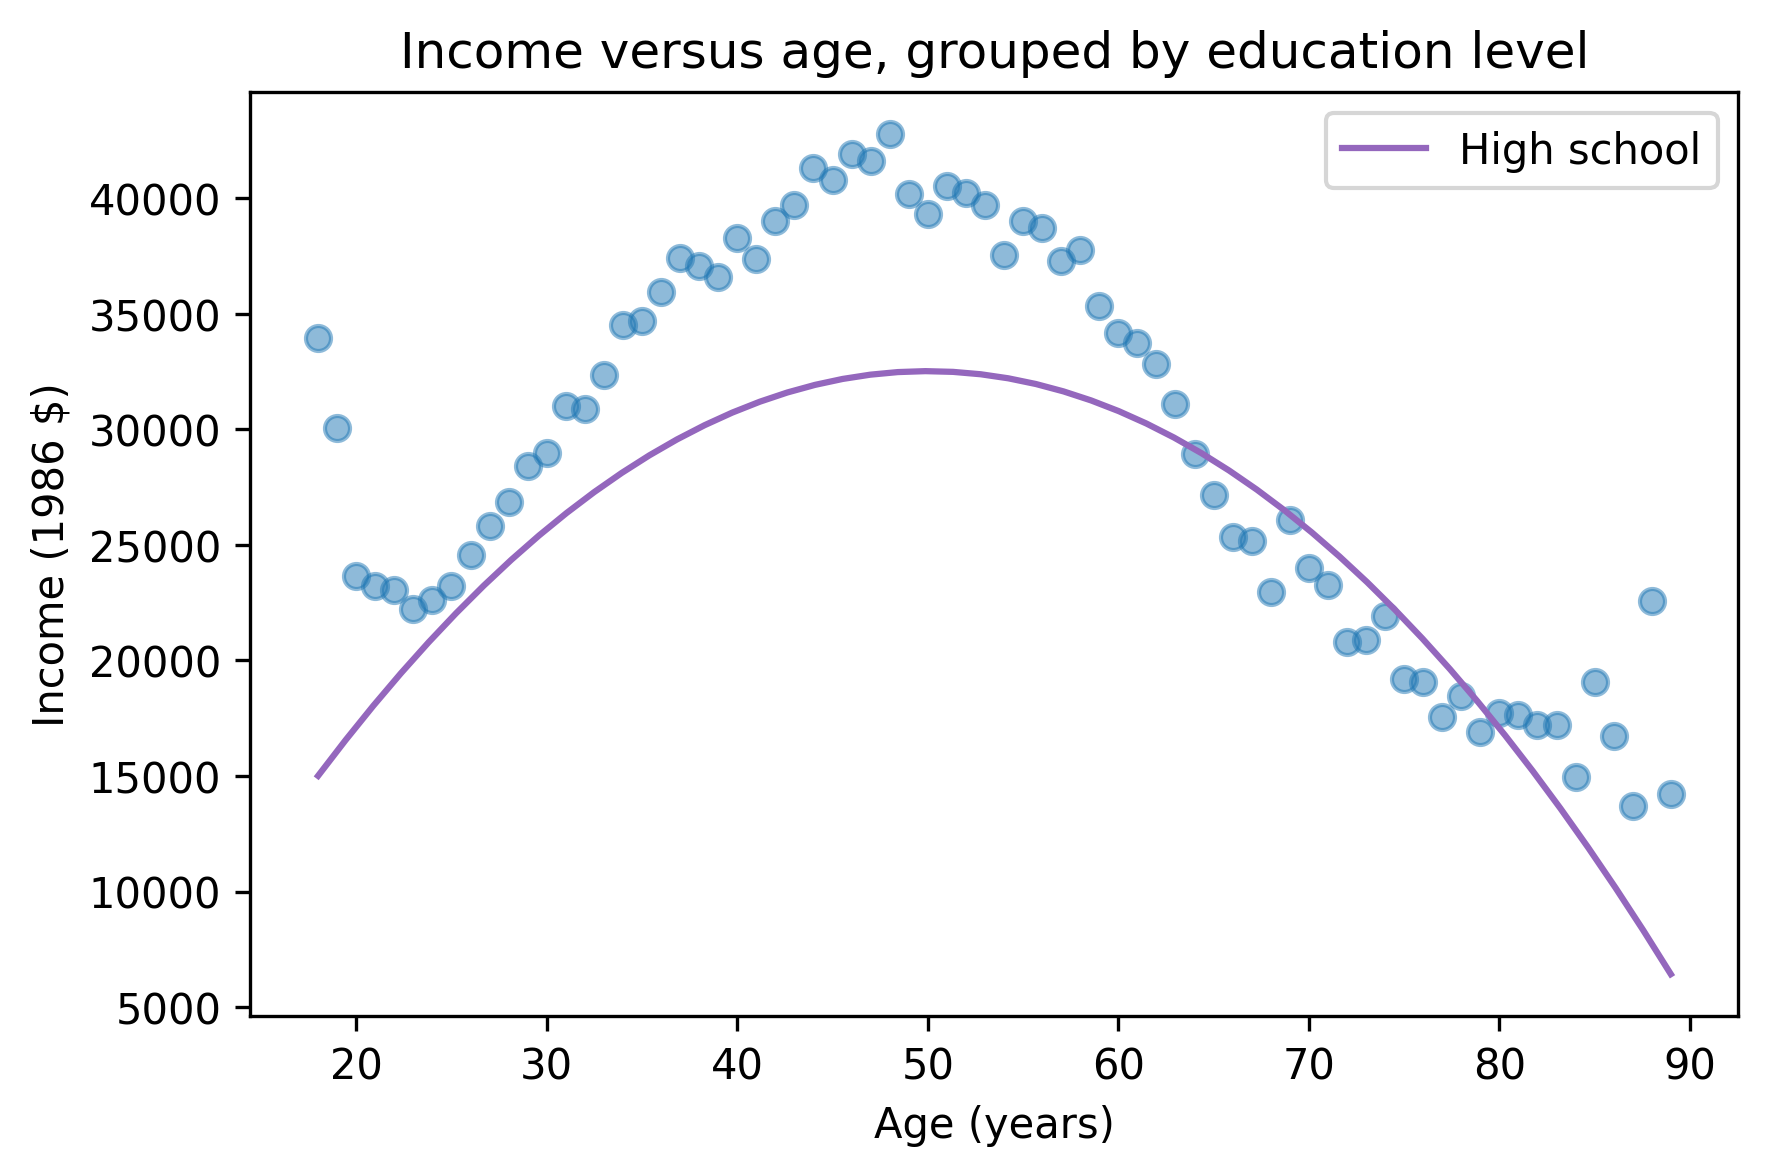
\includegraphics[width=4in]{chapters/10_regression_files/10_regression_53_0.png}
\end{center}

The lines show expected income as a function of age for three levels of
education. This visualization helps validate the model, since we can
compare the predictions with the data. And it helps us interpret the
model since we can see the separate contributions of age and education.

Sometimes we can understand a model by looking at its parameters, but
often it is better to look at its predictions. In the exercises, you'll
have a chance to run a multiple regression, generate predictions, and
visualize the results.

\textbf{Exercise:} At this point, we have a model that predicts income
using age, education, and sex.

Let's see what it predicts for different levels of education, holding
\passthrough{\lstinline!age!} constant.

\begin{itemize}
\item
  Create an empty \passthrough{\lstinline!DataFrame!} named
  \passthrough{\lstinline!df!}.
\item
  Using \passthrough{\lstinline!np.linspace()!}, add a column named
  \passthrough{\lstinline!educ!} to \passthrough{\lstinline!df!} with a
  range of values from \passthrough{\lstinline!0!} to
  \passthrough{\lstinline!20!}.
\item
  Add a column named \passthrough{\lstinline!educ2!} with the values
  from \passthrough{\lstinline!educ!} squared.
\item
  Add a column named \passthrough{\lstinline!age!} with the constant
  value \passthrough{\lstinline!30!}.
\item
  Add a column named \passthrough{\lstinline!age2!} with the values from
  \passthrough{\lstinline!age!} squared.
\item
  Use the \passthrough{\lstinline!results!} object and
  \passthrough{\lstinline!df!} to generate expected income as a function
  of education.
\end{itemize}

\textbf{Exercise:} Now let's visualize the results from the previous
exercise.

\begin{itemize}
\item
  Group the GSS data by \passthrough{\lstinline!educ!} and compute the
  mean income in each education group.
\item
  Plot mean income for each education group as a scatter plot.
\item
  Plot the predictions from the previous exercise.
\end{itemize}

How do the predictions compare with the data?

\hypertarget{categorical-variables}{%
\section{Categorical Variables}\label{categorical-variables}}

Most of the variables we have used so far -- like income, age, and
education -- are numerical. But variables like sex and race are
\textbf{categorical} -- that is, each respondent belongs to one of a
specified set of categories. If there are only two categories, the
variable is \textbf{binary}.

With StatsModels, it is easy to include a categorical variable as part
of a regression model. Here's an example:

\begin{lstlisting}[language=Python,style=source]
formula = 'realinc ~ educ + educ2 + age + age2 + C(sex)'
results = smf.ols(formula, data=gss).fit()
results.params
\end{lstlisting}

\begin{lstlisting}[style=output]
Intercept       -24635.767539
C(sex)[T.2.0]    -4891.439306
educ              -496.623120
educ2              156.898221
age               1720.274097
age2               -17.097853
dtype: float64
\end{lstlisting}

In the formula string, the letter \passthrough{\lstinline!C!} indicates
that \passthrough{\lstinline!sex!} is a categorical variable. The
regression treats the value \passthrough{\lstinline!sex=1!}, which is
male, as the reference group, and reports the difference associated with
the value \passthrough{\lstinline!sex=2!}, which is female. So the
results indicate that income for women is about \$4156 less than for
men, after controlling for age and education. However, note that
\passthrough{\lstinline!realinc!} represents household income. If the
respondent is married, it includes both their own income and their
spouse's. So we cannot interpret this result as an estimate of a gender
gap in income.

\hypertarget{logistic-regression}{%
\section{Logistic Regression}\label{logistic-regression}}

In the previous section, we added a categorical variables on the right
side of a regression formula -- that is, we used it as a predictive
variable.

But what if the categorical variable is on the left side of the
regression formula -- that is, it's the value we are trying to predict?
In that case, we can use \textbf{logistic regression}.

As an example, one of the GSS questions asks ``Would you favor or oppose
a law which would require a person to obtain a police permit before he
or she could buy a gun?'' The responses are in a column called
\passthrough{\lstinline!gunlaw!} -- here are the values.

\begin{lstlisting}[language=Python,style=source]
gss['gunlaw'].value_counts()
\end{lstlisting}

\begin{lstlisting}[style=output]
gunlaw
1.0    36367
2.0    11940
Name: count, dtype: int64
\end{lstlisting}

\passthrough{\lstinline!1!} means yes and \passthrough{\lstinline!2!}
means no, so most respondents are in favor. To explore the relationship
between this variable and factors like age, sex, and education, we can
use StatsModels, which provides a function that does logistic
regression. To use it, we have to recode the dependent variable so
\passthrough{\lstinline!1!} means ``yes'' and
\passthrough{\lstinline!0!} means ``no''. We can do that by replacing
\passthrough{\lstinline!2!} with \passthrough{\lstinline!0!}.

\begin{lstlisting}[language=Python,style=source]
gss['gunlaw'].replace([2], [0], inplace=True)
\end{lstlisting}

Now we can run the regression. Instead of
\passthrough{\lstinline!ols()!}, we'll use
\passthrough{\lstinline!logit()!}, which is named for the logit
function, which is related to logistic regression.

\begin{lstlisting}[language=Python,style=source]
formula = 'gunlaw ~ age + age2 + educ + educ2 + C(sex)'
results = smf.logit(formula, data=gss).fit()
\end{lstlisting}

\begin{lstlisting}[style=output]
Optimization terminated successfully.
         Current function value: 0.544026
         Iterations 5
\end{lstlisting}

Estimating the parameters for the logistic model is an iterative
process, so the output contains information about the number of
iterations. Other than that, everything is the same as what we have seen
before. Here are the estimated parameters.

\begin{lstlisting}[language=Python,style=source]
results.params
\end{lstlisting}

\begin{lstlisting}[style=output]
Intercept        1.483746
C(sex)[T.2.0]    0.740717
age             -0.021274
age2             0.000216
educ            -0.098093
educ2            0.005557
dtype: float64
\end{lstlisting}

The parameters are in the form of \textbf{log odds} -- I won't explain
them in detail here, except to say that positive values make the outcome
more likely and negative values make the outcome less likely. For
example, the parameter associated with \passthrough{\lstinline!sex=2!}
is \passthrough{\lstinline!0.74!}, which indicates that women are more
likely to support this form of gun control.

To see how much more likely, we can generate predictions, as we did with
linear regression. As an example, we'll generate predictions for
different ages and sexes, with education held constant. First we need a
\passthrough{\lstinline!DataFrame!} with a range of values for
\passthrough{\lstinline!age!} and a fixed value of
\passthrough{\lstinline!educ!}.

\begin{lstlisting}[language=Python,style=source]
df = pd.DataFrame()
df['age'] = np.linspace(18, 89)
df['educ'] = 12
\end{lstlisting}

Then we can compute \passthrough{\lstinline!age2!} and
\passthrough{\lstinline!educ2!}.

\begin{lstlisting}[language=Python,style=source]
df['age2'] = df['age']**2
df['educ2'] = df['educ']**2
\end{lstlisting}

We can generate predictions for men like this.

\begin{lstlisting}[language=Python,style=source]
df['sex'] = 1
pred_male = results.predict(df)
\end{lstlisting}

And for women like this.

\begin{lstlisting}[language=Python,style=source]
df['sex'] = 2
pred_female = results.predict(df)
\end{lstlisting}

Now, to visualize the results, we'll start by plotting the data. As
we've done before, we'll divide the respondents into age groups and
compute the mean in each group. The mean of a binary variable is the
fraction of people in favor. Then we can plot the predictions.

\begin{lstlisting}[language=Python,style=source]
grouped = gss.groupby('age')
favor_by_age = grouped['gunlaw'].mean()
plt.plot(favor_by_age, 'o', alpha=0.5)

plt.plot(df['age'], pred_female, label='Female')
plt.plot(df['age'], pred_male, '--', label='Male')

plt.xlabel('Age')
plt.ylabel('Probability of favoring gun law')
plt.title('Support for gun law versus age, grouped by sex')
plt.legend();
\end{lstlisting}

\begin{center}
\includegraphics[width=4in]{chapters/10_regression_files/10_regression_79_0.png}
\end{center}

According to the model, people near age 50 are least likely to support
gun control (at least as this question was posed). And women are more
likely to support it than men, by about 15 percentage points.

Logistic regression is a powerful tool for exploring relationships
between a binary variable and the factors that predict it. In the
exercises, you'll explore the factors that predict support for
legalizing marijuana in the U.S.

\textbf{Exercise:} In the GSS dataset, the variable
\passthrough{\lstinline!grass!} records the answer to the question ``Do
you think the use of marijuana should be made legal or not?'' Let's use
logistic regression to explore relationships between these responses and
age, sex, and education level.

\begin{enumerate}
\def\labelenumi{\arabic{enumi}.}
\item
  First, use \passthrough{\lstinline!replace!} to recode the
  \passthrough{\lstinline!grass!} column so that
  \passthrough{\lstinline!1!} means yes and \passthrough{\lstinline!0!}
  means no. Use \passthrough{\lstinline!value\_counts!} to check.
\item
  Next, use \passthrough{\lstinline!smf.logit()!} to predict
  \passthrough{\lstinline!grass!} using the variables
  \passthrough{\lstinline!age!}, \passthrough{\lstinline!age2!},
  \passthrough{\lstinline!educ!}, and \passthrough{\lstinline!educ2!},
  along with \passthrough{\lstinline!sex!} as a categorical variable.
  Display the parameters. Are men or women more likely to support
  legalization?
\item
  To generate predictions, start with an empty DataFrame. Add a column
  called \passthrough{\lstinline!age!} that contains a sequence of
  values from 18 to 89. Add a column called
  \passthrough{\lstinline!educ!} and set it to 12 years. Then compute a
  column, \passthrough{\lstinline!age2!}, which is the square of
  \passthrough{\lstinline!age!}, and a column,
  \passthrough{\lstinline!educ2!}, which is the square of
  \passthrough{\lstinline!educ!}.
\item
  Use \passthrough{\lstinline!predict!} to generate predictions for men
  (\passthrough{\lstinline!sex=1!}) and women
  (\passthrough{\lstinline!sex=2!}).
\item
  Generate a plot that shows (a) the average level of support for
  legalizing marijuana in each age group, (b) the level of support the
  model predicts for men as a function of age, and (c) the level of
  support predicted for women as a function of age.
\end{enumerate}

\hypertarget{summary}{%
\section{Summary}\label{summary}}

At this point, I'd like to summarize the topics we've covered so far,
and make some connections that might clarify the big picture. A central
theme of this book is \textbf{exploratory data analysis}, which is a
process and set of tools for exploring a dataset, visualizing
distributions, and discovering relationships between variables. The last
four chapters demonstrate the steps of this process:

\begin{itemize}
\item
  Chapter 7 is about importing and cleaning data, and checking for
  errors and other special conditions. This might not be the most
  exciting part of the process, but time spent understanding data can
  save you from embarrassing errors.
\item
  Chapter 8 is about exploring variables one at a time, visualizing
  distributions using PMFs, CDFs, and KDE, and choosing appropriate
  summary statistics.
\item
  In Chapter 9 we explored relationships between variables two at a
  time, using scatter plots and other visualizations; and we quantified
  those relationships using correlation and simple regression.
\item
  Finally, in this chapter, we explored multivariate relationships using
  multiple regression and logistic regression.
\end{itemize}

We moved through a lot of material quickly, but if you practice and
apply these methods to other questions and other datasets, you will
learn more as you go. In the next chapter, we will move on to a new
topic, resampling, which is a versatile tool for statistical inference.

